% ch: The application proposal
% INTRO = Stakeholder Requirements Specification (StRS)

% \citeonline{mengelkamp2018} -- read
% \citeonline{mihaylov2014} -- read -- used
% \citeonline{vangulick2018} -- read
% \citeonline{kounelis2017} -- read
% \citeonline{wang2018} -- read
% \citeonline{andoni2019} -- read -- to be used

The advent of \acrfullpl{dapp} in the whole electricity chain sector has been strengthening the integration of \glspl{ict} into the power network.
Despite the technology used so far has been enough to keep the infrastructure working through third-party services,
the blockchain enables a window of wisdom at the population level, where there is a big amount of low power customers mainly fed by one source, the distribution utility.

Moreover, aware that the Brazilian \acrfull{gd} legislation is inclined to the blockchain business model,
and the expected expansion of \acrfull{der} as a consequence of consumers looking for lower tariffs and renewable power energy,
the application purpose is to allow the trade of electricity within a community that shares the responsibility of managing their own power generation for self-consumption without relying on a third-party to do so.
%Excelente paragrafo

The community scope is the group of shareable consumption, i.e., enterprises of multiple consumer units (condominiums) and shareable generation (consortiums or cooperatives).
The members of the community range from power consumers to prosumers.
Although they can't sell back their surplus generation to the power utility, they can determine the rules to transfer electricity among the group.
This measurement follows both the group self ambitions and the local legislation guidelines.
Therefore, each member has a quota from the group power generation which represents the member ownership over a given energy portion.
And it is up to the member her/himself to determine how she/he would like to distribute her/his portion.

In order to keep the group objectives of sharing the power generation and the costs to do so as a priority, without be limited by trust factors due to members nature or bad system behaviour, the proposal suggests that any modification on the current quota distribution should be made in function of a token common for the whole group.
The token represents the group digital currency and its feasibility is guaranteed by the blockchain network.
This method gets rid of mistrust, gives transparency for the whole group about any quota change, and allows a safety inspection with updated values for the utility and the legislative bodies.

Such as \gls{ico}'s initiatives, the tokens of the group have a particular method to be created.
In the present case, every time a new power plant is added into the group power capacity, a new equivalent crypto-currency amount is created.
This methodology keeps the market simple when considering the new power plants and the variety of members on each investment round.
The token issued has a low variability on the intra-market because it is proportionally created by power units, and its purpose is to exchange energy solely.
However, the cost of each power unit relies on the power plant cost to generate that energy, that depends on different weather and fund scenarios.
This makes the market unique for each member, i.e., it is up to each member's strategic vision the decision to invest in new power plants or to exchange her/his quota to get profits beyond any investment made to only cover her/his power consumption.

This kind of crypto-currency is also referred to as a non-fungible token%
\footnote{\url{https://en.wikipedia.org/wiki/Non-fungible_token}} (NFT)
because it can not be interchangeable with the blockchain native assets but works well for specific use cases.
This approach is similar to the NRGcoin~\cite{mihaylov2014} in which tokens are created by raising the power generation capacity in the distribution grid, instead of spending energy on computational power to do so.
Curiously, new power plants will emerge only when desired by members to feed their electricity needs.
So, what makes the dynamic of the internal market is the growth of members and their financial investment capacity (and interest) to fund new distributed power plants.

Therefore, there is no need to store money to exchange back the tokens to fiat currency, because each token represents individual money savings by the difference between the tariffs of the group and the utility.
Thus, the income happens similarly to the energy credit process, i.e., each member gets her/his savings after a month-round period.
And the \gls{gd} can be considered as an investment portfolio with periodic returns.
Based on those premises, the token is useful to exchange quotas without directly rely on fiat money.
%Excelente frase, tanto anterior quanto a proxima
It allows the group to determine its own valuation of the different power sources,
and it gives to each member the opportunity to speculate how much her/his quota worth at any given moment, i.e., how much she/he is inclined to accept to exchange the quota.
% A blockchain application to manage the transactions assures a reliable member-to-member deal and transparency to the group and to the power distribution utility about the updated quota values.

Finally, the proposed \gls{dapp} context can be detached into three main layers as shown by \autoref{fig:sys-lay}.
% They can be interpreted as well as the concepts presented by \autoref{fig:sys-as-is}, but with subject detailing.
The information network layer is the key part of the development because it redefines the information flux interaction that comes from both remaining layers.
So, the traditional information flux about the power grid network between consumers/prosumers and utility is unchanged, the power meter continues to register the electricity and send this information in a one-way direction.
Similarly happens to the business layer, where the fundamental practices of the group of shareable consumption keep the same, except by the information management supported by the blockchain advantages,
in what now everyone has reliable access to their counterpart members data, and a impartial communication channel to alter their quotas.

The link between both business and power networks through the information layer is the member her/himself because she/he is the only one with access to her/his electricity meter information and with write-permission to the blockchain network at the same time.
The member as a blockchain node is responsible to input the required measuring values in the information network (off-chain service) and to interact with its peers (on-chain service).

\begin{figure}[htbp]{\textwidth}
    \centering
    \frame{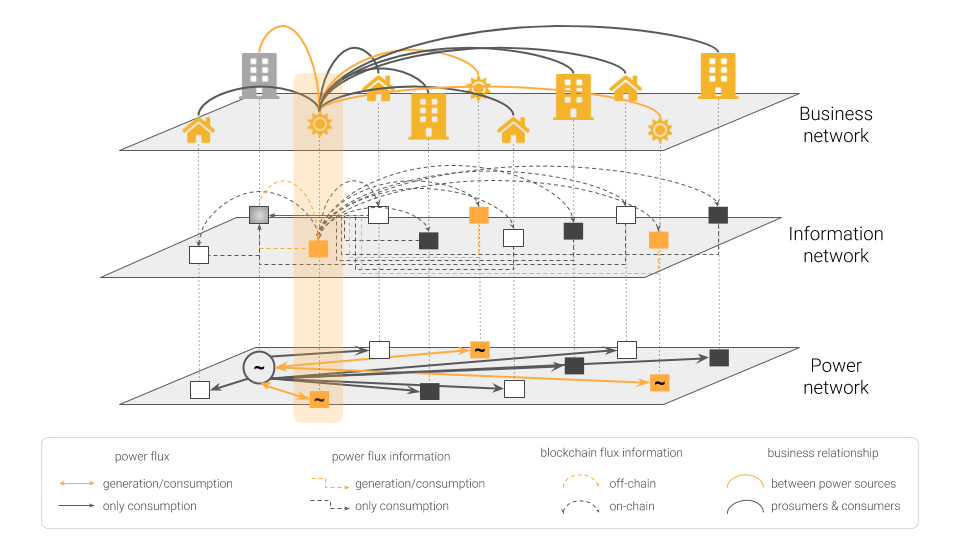
\includegraphics[width=\textwidth]{pics/dapp-op.png}} % fazer o desenho em slides primeiro e depois converter para tikz
    \caption{The operational layers of a micro/mini-grid and the blockchain approach on it from a prosumer point-of-view in a shareable generation group.}
    \label{fig:sys-lay}
    % \legend{}
    \source{Adapted from \citeonline{kounelis2017, andoni2019}.}
\end{figure}

Then, the proposed blockchain application is a small part of an entire management system to be used by the group of shareable consumption in the context of micro/mini-grid to offer to its members an intra-market to negotiate their electricity fraction earnings.
With support from the ISO/IEC/IEEE International Standard of Systems and software engineering -- Life cycle processes -- Requirements engineering (\citeyear{iso-iec-ieee}),
\autoref{sec:requisitos} describes the ordinary requirements for the \gls{dapp} developed.
The following \autoref{sec:platform} adds a comparison about some of the blockchains available on the market in order to justify the one used to develop the application.
\autoref{sec:the-dapp} presents the application itself,
and \autoref{sec:experiments} complements with a simulation about the application functionality making use of a real case of shareable consumption.

\section{Identification of the application requirements}
\label{sec:requisitos}

The design of an application requests the understanding of some system statements which captures the user needs, and associated constraints and conditions.
These requirements involve a set of specifications until reach the definitions of the software functions, performance, design constraints, and attributes~\cite{iso-iec-ieee}.
The \autoref{fig:sys-as-is} states the system approach of the whole process to develop a software, and highlight what the present work is up to advance toward a \gls{dapp}.

\def\c#1{\textbf{#1}}

\newcommand{\appschema}[4]{
\begin{figure}[h!btp]{\textwidth}
    \centering
    \caption{#1}
    {#2} % label
    
    % We need layers to draw the block diagram
    \pgfdeclarelayer{background}
    \pgfdeclarelayer{foreground}
    \pgfsetlayers{background,main,foreground}
    
    % Define a few styles and constants
    \tikzstyle{elemts}=[draw, fill=gray!20, text width=5em, text centered, minimum height=2.5em]
    \tikzstyle{target} = [draw, fill=gray!50, text width=6em, text centered, minimum height=2.5em, rounded corners]
    \tikzstyle{geral} = [rounded corners, draw=black!90]
    % \tikzstyle{ann} = [above, text width=5em]
    \tikzstyle{tbx} = [anchor=north west, text width=6em]
    % \def\blockdist{(-1,0.7)}
    \def\edgedist{(-0.2,0.2)}
    
    \def\bigtxt{\footnotesize{\c{market trends\\\medskip laws \& regulations}\\\medskip %
                legal liabilities\\\medskip social responsibilities\\\medskip \c{technology base}\\\medskip labor pool\\\medskip competing products\\\medskip \c{standards \& specifications\\\medskip public culture\\\medskip physical/natural environment}}}
    \def\bigtx{\footnotesize{policies \& procedures\\\medskip standards \& specifications\\\medskip %
                guidelines\\\medskip domain technologies\\\medskip local culture}}
    \def\bigt{\footnotesize{\c{business operational processes\\\medskip  business operational constraints}\\\medskip %
                business operational policies \& rules\\\medskip business operational modes\\\medskip business operational quality\\\medskip business structure}}
    
    \frame{%
    \resizebox{\textwidth}{!}{%
    \begin{tikzpicture}
        % general boxes
        % \node 
        \node (sftwr) [target] {Software\\(Dapp)};
        \node (sysel) [above of=sftwr] {System Element};
        \path [above of=sysel]+(0,1.5) node (elemt1) [elemts, text width=8em] {System Element};
        
        % titles
        \node (SYS) [above of=elemt1] {System};
        \path (SYS.north west)+(0,0.7) node (sysop) {System Operation};
        \path (sysop.north west)+(-2,0.7) node (bizop) {Business Operation};
        \path (bizop.north west)+(-0.5,0.7) node (orgen) {Organization Environment};
        \path (orgen.north west)+(-1.5,0.7) node (exten) {External Environment};
        
        % text boxes
        \path (bizop.south west)+(0,-0.25) node [tbx, text width=8em] {\bigt};
        \path (orgen.south west)+(0,-0.25) node [tbx] {\bigtx};
        \path (exten.south west)+(0,-0.25) node [tbx, text width=7em] {\bigtxt};
        
        % boxes of the titles
        \begin{pgfonlayer}{background}
            % External Environment
            \path (exten.north west)+\edgedist node (a) {};
            \path (sftwr.south -| sftwr.east)+(2,-1.2) node (b) {};
            \path[geral, draw=white] (a) rectangle (b);
            
            % Organization Environment
            \path (orgen.north west)+\edgedist node (a) {};
            \path (b)+(-0.2,0.2) node (b) {};
            \path[geral] (a) rectangle (b);
            
            % Business Operation
            \path (bizop.north west)+\edgedist node (a) {};
            \path (b)+(-0.2,0.2) node (b) {};
            \path[geral] (a) rectangle (b);
            
            % System Operation
            \path (sysop.north west)+\edgedist node (a) {};
            \path (b)+(-0.2,0.2) node (b) {};
            \path[rounded corners, draw=black!90, dashed] (a) rectangle (b);
            
            % System
            \path (sysel.west |- SYS.north)+(-0.4,0.2) node (a) {};
            \path (sftwr.south -| sysel.east)+(+0.4,-0.4) node (b) {};
            \path[geral] (a) rectangle (b);
            
            % System Element (of Dapp)
            % \path (sysel.north west)+(-0.2,0.2) node (a) {};
            % \path (sftwr.south -| sysel.east)+(+0.2,-0.2) node (b) {};
            % \path[elemts] (a) rectangle (b); % node 'System Element' with 'Software'
            \path let \p1=($(elemt1.west)-(elemt1.east)$), \n1 = {veclen(\p1)-\pgflinewidth},
                \p2=($(sysel.north)-(sftwr.south)$), \n2 = {veclen(\p2)} % -\pgflineheight
                in node[draw, elemts, minimum width=\n1, minimum height={1em+\n2}] at (0,0.4) (nome) {};
        \end{pgfonlayer}
    \end{tikzpicture}
    }}

    \legend{#3}
    \source{#4}
\end{figure}
}
\appschema{Concepts for the development of a system.}%
            {\label{fig:sys-as-is}}%
            {The grayer box and the bold texts highlight the propositions considered for the blockchain application development.}%
            {Adapted from \citeonline[fig.~4]{iso-iec-ieee}}

The different sets of requirement information items shown the broad range of knowledge to be considered for a fully decentralized system development.
Notwithstanding, the identification of each item requires interaction and cooperation among stakeholders, mainly to define how they interact through sets accordingly with business and system specifications.

The \autoref{fig:sys-as-is} presents the development scope from the top level environments, to the business level, to the ``specific system-of-interest''~\cite{iso-iec-ieee}.
The first addresses the external directives the system must follow, and some of the items had already been discussed (bold texts).
The second refers to the intended way of doing business, and the systems are mainly viewed as black-boxes. It is up to the group's guidelines and rules, and most of its items are out of the scope of the present work. The proposal considers only what may be universal for this business category.
At the third lays the user's viewpoint to interact with the aforementioned layers~\cite{iso-iec-ieee}.

% \section{System Requirements Specification (SyRS)}
Even not aware about all specifications, the core concept of the application can be developed with no additional issues.
In the future, the remaining features may improve the application presented here.
For instance, the definitions about how the registering of members will be conducted and how the user interface will be are out of the core of the application, i.e., the purpose to securely allow the transaction between members in a doubtful environment.

The case where the \gls{dapp} rely on off-chain platforms, such as the power meter or electricity bill of the members to gather the values from generation to input in the blockchain is another exception.
For both methods, the group guidelines must address what should be done to solve possible problems to access the information or if a violation is found.
Although a smart-contract can be held to deal with them, the subjects related to errors and penalties are out-of-bounds.

% \subsection{User requirements}
However, for sure, the application must be accessible in any device and the user experience must encompass a wide audience age.
The usability to request or to send tokens must be as easy as to send a text message,
and it may be provided by the blockchain platform chosen throughout the features available for the development.
Although it is an important aspect of the \gls{dapp} project design, the considered development is a hidden layer of the front-end project, which is not instigated.

Moreover, all the users must provide the same registration data available on their electricity bill at the first access to the blockchain environment of a particular group.
This constitutes sensitive data and it will be hidden from the public ledger.
Indeed, this process represents the step in which a user becomes a member of a group.
So, members may access those data but users not.

% \subsection{Project Constraints}
For what concerns members data, there is special attention to where members reside and if they pertain to the same power utility.
Although they could be in the same geographic area, this not implies being fed by the same distribution grid.
It is not restricted to form a group with those customers, but a transaction between them is.
Thus, each member must be classified by power utility in order to exchange tokens.

In addition, some mistakes may happen during a quota transaction,
for example one could type 100 instead of 10 when writing up her/his clause.
In other cases, get rid of the quota should be mandatory by legislation force.
As the group has a representative body to act on their behalf,
the application must allow corrective transaction to interfere on these issues accordingly to the group guidelines to do so.
It is important to remember that blockchain ledger is an append-only database, so a new transaction must be held to take its effect.
This measure doesn't compromise privacy, neither security, but guarantees a safe interference for its members.
However, to simplify, the group representation by members hierarchy was replaced by a voting process to validate the changing of any group asset.

% \paragraph{Stakeholders}
Lastly, the stakeholders involved in the system are:
\begin{enumerate*}[label={(\roman*)}]
    \item\label{con} consumers,
    \item\label{pro} prosumers,
    \item\label{pou} power utility, and
    \item\label{leg} legislator.
\end{enumerate*}
The \ref{con} and the \ref{pro} are represented by the basic role of a member of a given group.
They are the unique users of the application, and they can interchange position.
In a more common way, the former can become the latter, but the opposite is not impossible to happen.
The \ref{pou} and the \ref{leg} can read the public ledger to follow the changes in the quota, but they can't directly interact with the application.
For these ones, each member is only a hash number (the public key) which is cross-referenced on their own private database to get full identification.

For the sake of simplicity, the proposal considers that a member joins only one group, but no restriction was imposed in the code lines.
So, two members who reside in the same geographic area and who are fed by the same distribution utility may be or not part of the same group of shareable generation.

In summary, \autoref{appen:terms} gathers the terms that will be used throughout the publishing in addition to what has been presented so far.
Note that they do not represent the variables names, although they have been used to give readability for the code.
The application comprehension was designed through a \gls{uml} class diagram detailed in \autoref{appen:uml}.
There can be noticed the relationships and attributes of the \emph{reader}, the \emph{user} and the \emph{member}.
Similarly, the main concepts of the blockchain technology were detached to better identify the aforementioned application features.

% \noindent
% * How to guarantee veracity of inputed informations? \\
% ** can be changed over time by user or automatically gotten at utility system? \\
% *** The end value can be different by countability period, it will be later discussed... \\
% **** The special characteristics must be defined by cooperative rules.

\section{Choosing the right platform}
\label{sec:platform}

\subsection{Bitcoin}
\label{ssec:bitcoin}
% Bitcoin variation
    % Alguma aplicação acima?
    
% https://bitcoin.org/pt_BR/como-funciona
    
\subsection{Ethereum}
\label{ssec:ethereum}
% Ethereum
    % A maioria das aplicações apresentadas acima

\subsection{Neo}
\label{ssec:neo}
The Neo blockchain defines itself as a ``distributed network for the Smart Economy''~\cite{neowp}.
Based on the principle of digital identity, i.e., real identity information stamped in electronic form,
Neo allows a true physical asset ownership by means of a digital asset that can, in the near future, replace the Online Certificate Status Protocol (OCSP) to manage and record the X.509 Certificate Revocation List (CRL)~\cite{neowp}.
% "Our verification of identity when issuing or using digital identities includes the use of facial features, fingerprint, voice, SMS and other multi-factor authentication methods. At the same time, we will also use the blockchain to replace the Online Certificate Status Protocol (OCSP) to manage and record the X.509 Certificate Revocation List (CRL)."

The NEO blockchain digital assets has two forms of operation.
One known as global asset refers to the public system space, which involves the native assets NEO and GAS.
The other one refers to the contract assets that may follow some standards and usually have a private storage, an area created by a smart contract with restrictions to join in.
Although any new smart contract deployed on the public ledger can create its own private space, they have to follow  the NEP-5 standard (similar to Ethereum ERC-20) to keep compatibility over the whole system if they intend to create a side cryptocurrency.

Likewise most of blockchain technologies, Neo uses the native tokens to govern transactions.
The token NEO by itself represents the right to manage the network, such as voting for bookkeeping and involvement on network parameter changes.
Its value ranges from 1 to 100 million with integer steps, without subdivisions.
Its total amount was created in the genesis block and it was half divided between the supporters of NEO during the ICO and the NEO Council.
The latter manages the tokens in order to support ``NEO's long-term development, operation and maintenance and ecosystem'' and ``will not enter [into] the exchanges [processes]''~\cite{neowp}.
Therefore, who holds NEO tokens are part of the network owners and has right to manage the network by voting procedures.

The other token is the fuel to control the Neo network resources.
It is called NeoGas, abbreviated as just GAS, and has the same maximum total limit of 100 million, although its minimum unit is 0.00000001.
It is created proportionally to each NEO a peer has by a decay algorithm rate when a new block is generated.
It is used to charge transactions and smart contract operations, however some of them have no fee so far, such as those related to contract assets.
In addition, some NeoIDs have priority when a large amount of transactions happen, while others may get this benefit by paying additional GAS.

This option is valuable because the Neo consensus mechanism has a new block appending time of ... in average.
It is a quite good "waiting period" (tem um nome técnico pra isso!) compared to others \gls{dbft} blockchains, like ...
Furthermore, the distributed storage protocol utilizes the same technology used by IP management over the whole Internet, the Distributed Hash Table (DHT) technology. % VER com Igor!!
"Large files is divided into fixed-size data blocks that are distributed and stored in many different nodes."\cite{neowp}
Although this method impose a trade-off between redundancy and reliability, Neo aims to use token incentives and backbone nodes to solve it, so users may settle the requirements of a given file.
In the end, a file reliability level will be proportional to its assigned cost of store and access.

Moreover, the blockchain allows cross-chain interoperability through a protocol whose makes other smart contracts compatible with NeoContract system.
It is either possible to exchange tokens and to scatter the steps of a transaction across chains.

\textcolor{red}{Falar sobre as API's.}
 the API's to 'trackle' native and side cryptocurrencies over smart-contracts and transactions.
Since


\subsection{Tron?}
\label{ssec:tron}
% Tron

\subsection{Libra}
\label{ssec:libra}

There are many projects going on, one example is the Libra Blokchain, https://info.binance.com/en/research/marketresearch/libra.html, an alliance of JP Morgan, XXX , Facebook...

This blockchain will be used for xxx


\subsection{Hyperledger}
\label{ssec:hyperledger}

Different from the others, the Hyperledger is not a unique blockchain technology, but a family of \glspl{dlt} designed to fit diverse business requirements and allow cross-industry solutions.
It is an open source collaborative effort under the Linux Foundation with leaders in finance, banking, \gls{iot}, supply chains, manufacturing and technology~\cite{hyper1}.

Nonetheless, all the five frameworks available by the Hyperledger make use of a modular architectural design in order to ``encourage the re-use of common building blocks'', and to ``enable rapid innovation of the \gls{dlt} and the interfaces between them''~\cite{hyper2}.
Consequently it has the benefits of extensibility and flexibility,
allowing independent modification of any component in an interoperable way,
offering highly secure solutions through rich and easy-to-use \glspl{api}~\cite{hyper1, hyper2}.

Aware that business blockchain networks operates under a partial trust environment, and the requirements may represent a potentially unique optimization point for the technology~\cite{hyper2},
the resulting system design relies under the classification of permissioned blockchain network but the range between public and private definition varies by each characteristic of a specific framework.
Similarly, the whole family has a particular consensus method that not include the standard \gls{pow} with anonymous miners, neither the use of a native token nor a cryptocurrency~\cite{hyper1}.

The Hyperledger business modular approach is quite similar to what was shown at \autoref{fig:layers}.
Besides the consensus layer purpose (Layer 0), the remaining layers dive into business blockchain components of the generalized layers already presented.
For instance, the smart contract layer is part of the Layer 2a, but the provided data-stores module and identity services module can be correlated with the whole Layer 2.
Independently of where they stand -- on- or off-chain -- their purpose are to allow the better business fit by other modules.

In addition, there is a policy service module responsible for management of various system policies. It is a significant requirement to rule the application behaviour over all other modules, in this way it can be consistent with the Layer 5.
The \glspl{api} module concerns usability such as the Layer 4.
Another module is the interoperation itself (Layer 3), which supports interoperability between different blockchain instances.
The remaining modules can be correlated with the same layer.
The communication and crypto modules aims to allow ``peer-to-peer message transport between the nodes that participate in a shared ledger instance'' and ``different crypto algorithms or modules to be swapped out without affecting other modules''~\cite{hyper1}.
% mudar isso depois!

% Consensus
% FIGURE 1. GENERALIZED HYPERLEDGER CONSENSUS PROCESS FLOW --> diagrama de sequência

% "Hyperledger business blockchain frameworks reach consensus by performing two separate activities: 1. Ordering of transactions, and 2. Validating transactions"~\cite{hyper1}
% The former...
% The latter...

% When dealing with validations, it is more important to give special attention to logic errors than to syntax ones.
% For the latter, the transaction can be dropped with no significant consequences.
% But for the former, the ``errors are more complex and should be policy driven whether to continue processing or not, and we might want to log these transactions for auditing if the policy requires''~\cite{hyper1}.

Anyhow, four frameworks use a voting-based approach to consensus.
Hyperledger Fabric, Hyperledger Iroha and Hyperledger Indy by means of Apache Kafka, Sumeragi and Redundant Byzantine Fault Tolerance (RBFT), which are nothing than variations of \gls{pbft} method.
The Hyperledger Burrow uses \gls{pos} through Tendermint consensus engine\footnote{\href{https://github.com/hyperledger/burrow/}{https://github.com/hyperledger/burrow/}}.
Nonetheless, Hyperledger Sawtooth uses a lottery-based approach, the \gls{poet}~\cite{hyper1}.


% Transaction Dependencies
% "All four Hyperledger frameworks that support smart contracts assume that
% transactions are atomic.
% In other words, a transaction is considered either not yet started or else completed; a transaction cannot be partly completed.
% This ensures transaction integrity.
% When dependent actions (if this then that) must be committed together, some frameworks assume that the dependent actions are captured in a single smart contract.
% Others permit batching of transactions across multiple smart contracts.
% Thus, smart contracts can specify dependencies between multiple transactions which must be committed atomically.
% These references can be either implicit or explicit."~\cite{hyper2}

% "With an implicit reference, it is usually impossible to determine the order in which transactions must be applied.
% Bitcoin solves this by repeatedly trying to apply the transaction, which results in transactions being gradually executed as their prerequisites are satisfied.
% This behaviour requires a transaction staging component, such as mempool, which takes care of any expiring transactions the system could not apply.
% With an explicit reference, the user submitting the transactions specifies the ordering with some form of transaction identifiers.
% Just as implicit and explicit references impact the formation of the block, so does the dependency graph.
% The dependency graph can be either cyclic or acyclic, in other words, circular or non-circular.
% With cyclic dependencies, the entire group containing the cycle must be included in the same block.
% With acyclic dependencies, any portion of the sequence may be included in the block, as long as transactions are included according to the dependency graph.
% With implicit dependencies, cycles may be complex to resolve, which can prevent certain transactions from being validated in parallel and committed.
% On the other hand, explicit dependency references can allow for parallel execution of non-conflicting transactions within the same block."~\cite{hyper2}

% Smart Contracts in the Hyperledger Frameworks --> acho q tb não preciso falar sobre isso
% Fazer um resumão, pq não preciso disso tudo.
% Table 1. Smart Contract Implementations in Hyperledger Frameworks

\subsection{R3 Corda}
\label{ssec:r3corda}

% R3 Corda

% \subsection{Microsoft Azure} -- Não é uma solução da Microsoft, mas uma integração com a Hyperledger
% https://azure.microsoft.com/pt-br/solutions/blockchain/
% https://www.coindesk.com/microsoft-salesforce-join-hyperledger-enterprise-blockchain-consortium

\subsection{Comparison}

% Smart Contract Integrity and Availability
"To ensure the integrity and availability of the blockchain network and the smart contract layer, enterprise blockchains must control access to certain resources.
Since smart contracts are programs, they are vulnerable to malicious attack, coding errors, and poor design.
A breakdown in any of these areas can compromise the integrity or availability of the blockchain system."~\cite{hyper2}

"Business blockchain systems can apply time or token-based resource management techniques to ensure that any particular smart contract does not consume excessive resources."~\cite{hyper2}



% highlight features

% "However, for sure, the application must be accessible in any device and the user experience must encompasses a wide audience age.
% The usability to request or to send tokens must be as easy as send a text message,
% and it may be provided by the blockchain platform choosed."~(seção anterior)
% Quais API's estão disponíveis para facilitar isso?

% WHAT HAVE ALREADY BEEN DISCUSSED AND NEED TO BE IDENTIFIED AS FEATURES

% - technological compliance
%     - cost-effective
%     - fair
%     - robust
%     - flexibility

% - social compliance
%     - accessibility

% - blockchain application
%     - immutability
%     - non-repudiation
%     - integrity
%     - transparency
%     - equal rights

% - blockchain infrastructure
%     - scalability
%     - peer autonomy
%     - dynamic behaviour of peers (leave and join)
%     - self-organization
%     - decentralization
%     - fault-tolerance

% - permissionless OR permissioned
%     - consensus algorithm
%         - trust factor (how the consensus is met)
%         - computational power
%         - transaction speed
%     - main coin
%     - altcoin
%     - xu2017:
%         - cost efficiency
%         - performance
%         - number of failure points
%         - data/computation on/off chain

\begin{table}[h!tbp]{\textwidth}
    \centering
    \caption{To be defined...}
    \label{tab:comparison}
    \frame{% https://www.tablesgenerator.com/#

\begin{tabular}{m{2.8cm}lllllll}
                                            & \textbf{\nameref{ssec:bitcoin}} & \textbf{\nameref{ssec:ethereum}} & \textbf{\nameref{ssec:neo}} & \textbf{\nameref{ssec:tron}} & \textbf{\nameref{ssec:libra}} & \textbf{\nameref{ssec:hyperledger}} & \textbf{\nameref{ssec:r3corda}} \\
\multicolumn{8}{l}{\cellcolor[HTML]{C0C0C0}Technological Compliance}                                                                                                                                                                                                                                                                                                             \\
cost-effective                              & \multicolumn{1}{c}{}                         & \multicolumn{1}{c}{}                          & \multicolumn{1}{c}{}                     & \multicolumn{1}{c}{}                      & \multicolumn{1}{c}{}                       & \multicolumn{1}{c}{}                             & \multicolumn{1}{c}{}                         \\
fair                                        & \multicolumn{1}{c}{}                         & \multicolumn{1}{c}{}                          & \multicolumn{1}{c}{}                     & \multicolumn{1}{c}{}                      & \multicolumn{1}{c}{}                       & \multicolumn{1}{c}{}                             & \multicolumn{1}{c}{}                         \\
robust                                      & \multicolumn{1}{c}{}                         & \multicolumn{1}{c}{}                          & \multicolumn{1}{c}{}                     & \multicolumn{1}{c}{}                      & \multicolumn{1}{c}{}                       & \multicolumn{1}{c}{}                             & \multicolumn{1}{c}{}                         \\
flexibility                                 &                                              &                                               &                                          &                                           &                                            &                                                  &                                              \\
\multicolumn{8}{l}{\cellcolor[HTML]{C0C0C0}Social Compliance}                                                                                                                                                                                                                                                                                                                    \\
accessibility                               & \multicolumn{1}{c}{}                         & \multicolumn{1}{c}{}                          & \multicolumn{1}{c}{}                     & \multicolumn{1}{c}{}                      & \multicolumn{1}{c}{}                       & \multicolumn{1}{c}{}                             & \multicolumn{1}{c}{}                         \\
\multicolumn{8}{l}{\cellcolor[HTML]{C0C0C0}Blockchain Application}                                                                                                                                                                                                                                                                                                               \\
imutability                                 & \multicolumn{1}{c}{}                         & \multicolumn{1}{c}{}                          & \multicolumn{1}{c}{}                     & \multicolumn{1}{c}{}                      & \multicolumn{1}{c}{}                       & \multicolumn{1}{c}{}                             & \multicolumn{1}{c}{}                         \\
non-repudiation                             &                                              &                                               &                                          &                                           &                                            &                                                  &                                              \\
integrity                                   &                                              &                                               &                                          &                                           &                                            &                                                  &                                              \\
transparency                                &                                              &                                               &                                          &                                           &                                            &                                                  &                                              \\
equal rights                                &                                              &                                               &                                          &                                           &                                            &                                                  &                                              \\
\multicolumn{8}{l}{\cellcolor[HTML]{C0C0C0}Blockchain Infrastructure}                                                                                                                                                                                                                                                                                                            \\
scalability                                 & \multicolumn{1}{c}{}                         & \multicolumn{1}{c}{}                          & \multicolumn{1}{c}{}                     & \multicolumn{1}{c}{}                      & \multicolumn{1}{c}{}                       & \multicolumn{1}{c}{}                             & \multicolumn{1}{c}{}                         \\
peer autonomy                               & \multicolumn{1}{c}{}                         & \multicolumn{1}{c}{}                          & \multicolumn{1}{c}{}                     & \multicolumn{1}{c}{}                      & \multicolumn{1}{c}{}                       & \multicolumn{1}{c}{}                             & \multicolumn{1}{c}{}                         \\
dynamic behaviour of peers (leave and join) & \multicolumn{1}{c}{}                         & \multicolumn{1}{c}{}                          & \multicolumn{1}{c}{}                     & \multicolumn{1}{c}{}                      & \multicolumn{1}{c}{}                       & \multicolumn{1}{c}{}                             & \multicolumn{1}{c}{}                         \\
self-organization                           &                                              &                                               &                                          &                                           &                                            &                                                  &                                              \\
decentralization                            &                                              &                                               &                                          &                                           &                                            &                                                  &                                              \\
fault-tolerance                             &                                              &                                               &                                          &                                           &                                            &                                                  &                                              \\
\multicolumn{8}{l}{\cellcolor[HTML]{C0C0C0}Permissionless or Permissioned}                                                                                                                                                                                                                                                                                                       \\
consensus algorithm                         &                                              &                                               &                                          &                                           &                                            &                                                  &                                              \\
main coin                                   &                                              &                                               &                                          &                                           &                                            &                                                  &                                              \\
altcoin                                     &                                              &                                               &                                          &                                           &                                            &                                                  &                                              \\
\textit{cost efficiency}                    &                                              &                                               &                                          &                                           &                                            &                                                  &                                              \\
\textit{performance}                        &                                              &                                               &                                          &                                           &                                            &                                                  &                                              \\
\textit{number of failure points}           &                                              &                                               &                                          &                                           &                                            &                                                  &                                              \\
\textit{data/computation on/off chain}      &                                              &                                               &                                          &                                           &                                            &                                                  &                                             
\end{tabular}}
    % \legend{}
    % \source{}
\end{table}

\section{The Dapp specifications}
\label{sec:the-dapp}
% \section{The Dapp requirements specification}
% \section{The distributed application}
% \section{Software Requirements Specification (SRS)}

% "Ongoing discussions revolve around the following questions:
% - Who should own and operate a distribution-level market?
% - What should the market rules and product definitions look like?
% - How should wholesale- and retail-level energy markets interact?"
% - What are the costs and benefits of TE, really?"~\cite{masiello2016}

% "This article ~\cite{masiello2016} provides a good summary of the market and technology issues to be faced down each of two paths for implementation—should there be a hierarchy of wholesale-level independent service operators (ISOs) and retail-level DSOs or one big centralized market/system operator?"

The \gls{dapp} purpose is to allow members from a group of shareable consumption to safely interact to exchange their power assets and to give transparency to others about their transactions.
For this end, the application is composed by one smart contract responsible to define the group-centered blockchain environment apart of the main blockchain network.
This is important to protect members' data from public access and to guarantee the transactions only between them.

The developed smart contract, also called as \gls{mtemsm}, has several functions and restrictions to deal with different kinds of transaction.
Its has its own public address after being deployed on the main blockchain network.
From the system interface, any user can make a transaction with this smart contract address to invoke a specific function.
Note that it is not required to transfer \emph{NEO coins}, but a transaction fee in \emph{GAS} exist and must be payed by whoever request the transaction.
By the same interface, anyone can track the transactions results based on the publishing \emph{events} or any other return argument, from (dis)approval to join the group, to modifications on a member's dataset.

Although those types of information in the blockchain ledger can be accessible by everyone, some of them are restricted by user levels.
Thereby, any cryptographic result remains for public access while some general information about the group can be accessed through any user account, and the cross-referencing between real-world identification with the blockchain digital identity keeps accessible only to members.
\Autoref{fig:flow-mtemsm} presents an overview of the \gls{mtemsm} interface with three sets of operations, namely:
\begin{description} % emph
    \item[General] provides only one function for users to request to join the group.
    
    \item[Partially restricted] also provides only one function but with restrictions based on what information is requested. So members and users have different access by each statement provided, which can be about the group power capacity, the group number of members, a given power plant registration data, or a member dataset.
    
    \item[Restricted] provides the main functions for members to vote on a process, to bid on a power plant crowdfunding, or to transact between them. Moreover, some administrative functions are also available to handle off-chain operations. Neither of these functions is restricted by members hierarchy but any other user interaction will not be allowed.
\end{description}

\begin{figure}[h!tbp]{\textwidth}
    \centering
    \caption{Available functions organized by operations access over a transaction with the \gls{mtemsm}.}
    \label{fig:flow-mtemsm}
    \frame{\resizebox{\textwidth}{!}{\begin{tikzpicture}

    % Specification of nodes
    \node (s1)  []                                  {EVENTS};
    \node (s2)  [right=of s1]                       {GLOBAL VARIABLES};
    \node (s3)  [below=of s1.west, anchor=west]     {THE MAIN INTERFACE};
    
    \node (o1)    [onchain, below=of s3.west, anchor=west]  {General operation.};
    \node (o2)    [onchain, right=of o1]                    {Partially restricted operation.};
    \node (o3)    [onchain, right=of o2]                    {Restricted operations.};
    \node (o4)    [onchain, below=of o3, xshift=1.5cm]      {Group operations.};
    \node (o5)    [onchain, below=of o4]                    {Administrative operations.};
    
    \node (s4)  [below=of o1.west, anchor=west, yshift=-5cm]    {GROUP FUNCTIONS};
    \node (s5)  [right=of s4]                                   {SYSTEM FUNCTIONS};
    \node (s6)  [right=of s5]                                   {ADMINISTRATIVE FUNCTIONS};
    
    \node (s7)  [below=of s4.west, anchor=west]     {METHODS FOR MEMBERS};
    \node (s8)  [right=of s7]                       {METHODS FOR POWER PLANTS};
    \node (s9)  [right=of s8]                       {METHODS FOR REFERENDUMS};
    \node (s10) [below=of s9.east, anchor=east]     {METHODS TO FINANCE A NEW POWER PLANT (aka an ICO of a NFT)};
    
    % Identification of the system interface
    \draw (s3.north west) rectangle (o5.south east);
    
    % Identification of the system integration
    \draw[thick, dashed] (s1.north west) rectangle (s2.south east);
    \draw[thick, dashed] (s4.north west) rectangle (s6.south east);
    \draw[thick, dashed] (s7.north west) rectangle (s10.south east);
    
\end{tikzpicture}}}
    \source{\copyright}
\end{figure}

As initially observed, the \gls{dapp} does not cover all aspects to the management system but its core agents, objects and relationships are detailed in the UML diagram on \Autoref{appen:uml}.
This representation supports the development of the following functions related to the operations described above.
In addition, it is possible to get a broad view of the \gls{mtemsm} integration with the main blockchain network, its services, and off-chain interface.
It also has a member-centered approach to better handle with the system management purpose.

Moreover, three other specifications were considered throughout the \gls{dapp} development.
One concerns to financial subjects. So a lot of decisions are carefully taken before reach the final desired result in order to shrink the amount of GAS consumed.
This methodology is based on the suggestions provided by a post on \emph{Medium}%
\footnote{\href{https://medium.com/@gongxiaojing0825/practical-tips-in-developing-neo-smart-contract-a872a4f910c1}{Practical Tips in Developing NEO Smart Contracts}},
and on the computing expenses table at NEO blockchain system%
\footnote{\href{https://docs.neo.org/docs/en-us/sc/fees.html}{NEO System Fees}}.

The other concerns to the NeoVM limitations to compile the full C# library.
For instance, most of C# integral types are converted to \verb|BigInteger| type in the NeoVM.
So, initially, the \gls{mtemsm} was designed with only the variables types allowed by the compiler.
However, the cost to storage a \verb|byte| (\verb|unit8|) variable is ..., even been converted to \verb|BigInteger|.
While a ``native'' \verb|BigInteger| variable will always cost ...
This way, a more detailed definition of the variables types were considered to better handle with an economic development.
And it has also supported a better description of the code.

The last specification is the time stamp format used, a important variable to deal on a distributed environment.
NEO system uses Unix time stamp to synchronize its operations.
It represents the date and hour running time in seconds since January 1st, 1970 at UTC%
\footnote{\href{https://en.wikipedia.org/wiki/Unix_time}{Unix time}}.
Therefore, all constants and variables of time were defined in this format.
Even the time frames considered are multiple of seconds, for instance a 30 days period has a constant value of 259200 seconds.
And none time conversion was implemented to deal with input variables different from this format because it must be handled off-chain.

At a glance, each of the developed functions behaviours are described in the following subsections.
The pseudo-codes catch all cases when faced with any kind of input, from how it is processed, to how the output is generated.



%------------------------------------------------------
% 10. External interfaces - Define all inputs into and outputs from the software system. The description should complement the interface descriptions in 9.5.3.3.1 through 9.5.3.3.5, and should not repeat information there.
% Each interface defined should include the following content:
% Jmen caliss para os inputs!
% COLOCAR NOS \paragraph{}
% Necessário detalhar como são as notificações, publicações de eventos e registros na blockchain!

% 11. Functions - Define the fundamental actions that have to take place in the software in accepting and processing the inputs and in processing and generating the outputs, including
% COLOCAR NOS \paragraph{}

\subsection*{Function \texttt{admission}}

It is the entry way to the group environment to share the benefit and cost of a \gls{gd}.

Any user can make a transaction with the \gls{mtemsm} address through the function \verb|Admission| to request to join the group.
...

To take part of it, a NEO user must request access to the group environment through a transaction with the related smart contract address.
After the approval, the user is identified inside the group and can make use of other functions and smart contracts belonging to this private environment.
\autoref{fig:flow-mtemsm} shows this workflow and at \autoref{appen:2} is the related smart contract code.

Furthermore, after an approval, the \gls{mtemsm} stores the member personal data on the internal smart contract memory space, and hence, the member could access other functions to interact with other members.

\hline

\gls{mem} is the class which managers each member registering data, both personal and ``economic'' ones.
It has the functions to check the individual balance of tokens and the shares of the group's power.
It also has an option to get the most updated values from a member or from the whole group all at once.

\begin{figure}[h!tbp]{\textwidth}
    \centering
    \caption{A user point-of-view process to be accepted in a group's private environment.}
    \label{fig:flow-admision}
    \frame{\resizebox{\textwidth}{!}{\begin{tikzpicture}

    % Specification of nodes
    \node (start) [terminal]                    {Activity starts.};
    
    \node (d1)    [decision, below=of start]    {Were all the required inputs provided?};
    \node (d2)    [decision, below=of d1]       {Does the address provided belong to the invoker?};
    \node (d3)    [decision, below=of d2]       {Is the invoker already a member?};
    
    \node (e1)    [i-o, right=of d2]            {Displays an error message.};
    
    \node (o1)    [onchain, below=of d3]        {Gets the inputs provided.};
    \node (o2)    [onchain, below=of o1]        {Creates and stores an ID for follow-up.};
    
    \node (e2)    [i-o, right=of o2]            {Displays the request from the invoker.};
    \node (e3)    [i-o, right=of e2]            {Returns the ID.};
    
    \node (o3)    [offchain, right=of e3]       {Waits a time frame period to keep going.};
    \node (o4)    [onchain, below=of o3]        {During a time frame, members can vote on this ID.};
    \node (o5)    [onchain, right=of o3]        {Any member resumes the process.};
    
    \node (d4)    [decision, above=of o5]       {Was the ID provided?};
    \node (d5)    [decision, above=of d4]       {Did the time frame pass out?};
    
    \node (o6)    [onchain, right=of d5]        {Calculates the result.};
    
    \node (d6)    [decision, above=of o6]       {Is the membership request approved?};
    
    \node (o7)    [onchain, right=of d6]        {Stores the new member dataset.};
    
    \node (e4)    [i-o, above=of d6]            {Displays the disapproval.};
    \node (e5)    [i-o, right=of e4]            {Displays the approval.};
    
    \node (end)   [terminal, above=of e4]       {Activity ends.};


    % Specification of lines between nodes defined above with additional nodes for description.
    \draw[->]  (start) -- (d1);
    \draw[->]     (o1) -- (o2);
    \draw[->]     (o2) -- (e2);
    \draw[->]     (e2) -- (e3);
    \draw[->]     (e3) -- (o3);
    \draw[->]     (e3) |- (o4);
    \draw[->]     (o3) -- (o5);
    \draw[->]     (o5) -- (d4);
    \draw[->]     (o6) -- (d6);
    \draw[->]     (o7) -- (e5);
    \draw[->]     (e4) -- (end);
    \draw[->]     (e5) |- (end);

    \draw[->]     (d1) -- node[left=2.5mm]  {Yes} (d2);
    \draw[->]     (d2) -- node[left=2.5mm]  {Yes} (d3);
    \draw[->]     (d4) -- node[left=2.5mm]  {Yes} (d5);
    \draw[->]     (d5) -- node[above=2.5mm] {Yes} (o6);
    \draw[->]     (d6) -- node[above=2.5mm] {Yes} (o7);
    \draw[->]     (d3) -- node[left=2.5mm]  {No}  (o1);
    \draw[->]     (d2) -- node[above=2.5mm] {No}  (e1);
    \draw[->]     (d6) -- node[left=2.5mm]  {No}  (e4);
    \draw[->]     (d1) -| node[pos=0.25, above=2.5mm] {No}  (e1);
    \draw[->]     (d3) -| node[pos=0.25, above=2.5mm] {Yes} (e1);
    \draw[->]     (d4) -| node[pos=0.25, above=2.5mm] {No}  (e1);
    \draw[->]     (d5) -| node[pos=0.25, above=2.5mm] {No}  (e1);
    
    \draw[->]     (e1) -- ++(4cm,0) |- (end) node {};
    
\end{tikzpicture}}}
    \source{\copyright}
\end{figure}

\subsection*{Function \texttt{summary}}

\begin{figure}[h!tbp]{\textwidth}
    \centering
    \caption{The process to get information from the group.}
    \frame{\resizebox{0.5\textwidth}{!}{\begin{tikzpicture}

    % Specification of nodes
    \node (start) [terminal]                    {Activity starts.};
    
    \node (d1)    [decision, below=of start]    {Were all the required inputs provided?};
    \node (d2)    [decision, below=of d1]       {Is the invoker not a member and the ID argument an address?};
    
    \node (e1)    [i-o, right=of d1]            {Displays an error message.};
    
    \node (o1)    [onchain, below=of d2]        {Gets the inputs provided.};
    
    \node (d3)          [decision, below=of o1]       {Is the \emph{key} a member address?};
        \node (d4)      [decision, right=of d3]       {Is the optional argument empty?};
            \node (e2)  [i-o, right=of d4]            {Returns a member's dataset information.};
        \node (d5)      [decision, below=of d4]       {Is the optional argument equal to \verb|"detailed"|?};
            \node (e3)  [i2o, right=of d5]            {Returns a member's dataset information and all PP IDs she/he has a quota on.};
        \node (o2)      [onchain, below=of d5]        {The optional argument is equal to something else.};
        \node (e4)      [i-o, right=of o2]            {Returns the respective information stored.};
    
    
    \node (d6)      [decision, left=of d3]       {Is the \emph{key} a PP ID?};
        \node (d7)  [decision, left=of d6]       {Is the PP operational?};
            
            % Yes, PP is operational.
            \node (d8)      [decision, left=of d7]      {Is the optional argument empty?};
                \node (e5)  [i-o, left=of d8]           {Returns a PP's dataset information.};
            \node (d9)      [decision, below=of d8]     {Is the optional argument equal to \verb|"detailed"|?};
                \node (e6)  [i2o, left=of d9]           {Returns a PP's dataset information and all member addresses it has shares with.};
            \node (o3)      [onchain, below=of d9]      {The optional argument is equal to something else.};
            \node (e7)      [i-o, left=of o3]           {Returns the respective information stored.};
        
            % No, PP is not operational.
            \node (d10)     [decision, below=of d7, yshift=-10cm] {Is the optional argument empty?};
                \node (e8)  [i-o, left=of d10]                    {Returns a PP's crowdfunding information.};
            \node (d11)     [decision, below=of d10]              {Is the optional argument equal to \verb|"detailed"|?};
                \node (e9)  [i2o, left=of d11]                    {Returns a PP's crowdfunding information and all member addresses whose have bided on it if it has succeed.};
            \node (o4)      [onchain, below=of d11]               {The optional argument is equal to something else.};
            \node (e10)     [i-o, left=of o4]                     {Returns the respective information stored.};
    
    \node (d12)         [decision, below=of d3, yshift=-10cm]       {Is the \emph{key} a referendum ID?};
        \node (d13)     [decision, right=of d12]                    {Is the optional argument empty?};
            \node (e11) [i-o, right=of d13]                         {Returns a referendum's process information.};
        \node (o5)      [onchain, below=of d13]                     {The optional argument is equal to something else.};
        \node (e12)     [i-o, right=of o5]                          {Returns the respective information stored.};
    
    \node (o6)      [onchain, below=of d12, yshift=-5cm]        {The \emph{key} is equal to something else.};
    \node (e13)     [i-o, right=of o6]                          {Returns a summary of the group.};
    
    \node (end)   [terminal, below=of e13, yshift=-4cm]       {Activity ends.};
    
    \node[right=of end, xshift=8cm] (ref1) {};
    \node[left=of end, xshift=-28cm] (ref2) {};

    % Specification of lines between nodes defined above with additional nodes for description.
    \draw[->] (start) -- (d1);
    \draw[->]    (o1) -- (d3);
    \draw[->]    (o2) -- (e4);
    \draw[->]    (o3) -- (e7);
    \draw[->]    (o4) -- (e10);
    \draw[->]    (o5) -- (e12);
    \draw[->]    (o6) -- (e13);

    \draw[->]     (d1) -- node[left=2.5mm]  {Yes} (d2);
    \draw[->]     (d2) -- node[left=2.5mm]  {Yes} (o1);
    \draw[->]     (d3) -- node[above=2.5mm] {Yes} (d4);
    \draw[->]     (d4) -- node[above=2.5mm] {Yes} (e2);
    \draw[->]     (d5) -- node[above=2.5mm] {Yes} (e3);
    \draw[->]     (d6) -- node[above=2.5mm] {Yes} (d7);
    \draw[->]     (d7) -- node[above=2.5mm] {Yes} (d8);
    \draw[->]     (d8) -- node[above=2.5mm] {Yes} (e5);
    \draw[->]     (d9) -- node[above=2.5mm] {Yes} (e6);
    \draw[->]    (d10) -- node[above=2.5mm] {Yes} (e8);
    \draw[->]    (d11) -- node[above=2.5mm] {Yes} (e9);
    \draw[->]    (d12) -- node[above=2.5mm] {Yes} (d13);
    \draw[->]    (d13) -- node[above=2.5mm] {Yes} (e11);

    \draw[->]     (d1) -- node[above=2.5mm] {No}  (e1);
    \draw[->]     (d3) -- node[above=2.5mm] {No}  (d6);
    \draw[->]     (d4) -- node[left=2.5mm]  {No}  (d5);
    \draw[->]     (d5) -- node[left=2.5mm]  {No}  (o2);
    \draw[->]     (d7) -- node[left=2.5mm]  {No}  (d10);
    \draw[->]     (d8) -- node[left=2.5mm]  {No}  (d9);
    \draw[->]     (d9) -- node[left=2.5mm]  {No}  (o3);
    \draw[->]    (d10) -- node[left=2.5mm]  {No}  (d11);
    \draw[->]    (d11) -- node[left=2.5mm]  {No}  (o4);
    \draw[->]    (d12) -- node[left=2.5mm]  {No}  (o6);
    \draw[->]    (d13) -- node[left=2.5mm]  {No}  (o5);
    
    \draw[->]     (d2) -| node[pos=0.25, above=2.5mm] {No}  (e1);
    \draw[->]     (d6) |- node[pos=0.25, left=2.5mm]  {No}  (d12);
    
    \draw[->]    (e1) -| (ref1) -- (end);
    \draw[->]    (e2) -| (ref1) -- (end);
    \draw[->]    (e3) -| (ref1) -- (end) ;
    \draw[->]    (e4) -| (ref1) -- (end) ;
    \draw[->]    (e5) -| (ref2) -- (end);
    \draw[->]    (e6) -| (ref2) -- (end);
    \draw[->]    (e7) -| (ref2) -- (end) ;
    \draw[->]    (e8) -| (ref2) -- (end) ;
    \draw[->]    (e9) -| (ref2) -- (end) ;
    \draw[->]   (e11) -| (ref1) -- (end);
    \draw[->]   (e10) |- (end) ;
    \draw[->]   (e12) |- (end) ;
    \draw[->]   (e13) -- (end);
    
\end{tikzpicture}}}
    % \legend{}
    \source{\copyright}
\end{figure}

\subsection*{Function \texttt{bid}}

\begin{figure}[h!tbp]{\textwidth}
    \centering
    \caption{A general bid procedure during a new power plant crowdfunding process.}
    \frame{\resizebox{0.5\textwidth}{!}{\begin{tikzpicture}

    % Specification of nodes
    \node (start) [terminal]                    {Activity starts.};
    
    \node (d1)    [decision, below=of start]    {Were all the required inputs provided?};
    \node (d2)    [decision, below=of d1]       {Does the address provided belong to the invoker?};
    \node (d3)    [decision, below=of d2]       {Is the provided PP ID a valid one?};
    \node (d4)    [decision, below=of d3]       {Does the invoker belong to the same power utility as the PP under funding?};
    \node (d5)    [decision, below=of d4]       {Is it offered a factual value?};
    \node (d6)    [decision, below=of d5]       {Still time to bid?};
    
    \node (e1)    [i-o, right=of d3]            {Displays an error message.};
    
    \node (o1)    [onchain, below=of d6]        {Gets the inputs provided.};
    
    \node (d7)    [decision, right=of o1, xshift=2.4mm]       {Is the bid value greater than the remaining deal?};
    
    \node (o2)    [onchain, right=of d7]        {Increases the value gathered so far.};
    \node (o3)    [onchain, above=of o2]        {Increases the number of contributions.};
    \node (o4)    [onchain, above=of o3]        {Keeps an identified record of the bid.};
    
    \node (e2)    [i-o, above=of o4]            {Displays the bid statement.};
    \node (e3)    [i-o, above=of e2]            {Returns \verb|"true"|.};
    
    \node (end)   [terminal, above=of e3]       {Activity ends.};


    % Specification of lines between nodes defined above with additional nodes for description.
    \draw[->]  (start) -- (d1);
    \draw[->]     (o1) -- (d7);
    \draw[->]     (o2) -- (o3);
    \draw[->]     (o3) -- (o4);
    \draw[->]     (o4) -- (e2);
    \draw[->]     (e2) -- (e3);
    \draw[->]     (e1) -| (end);
    \draw[->]     (e3) -- (end);

    \draw[->]     (d1) -- node[left=2.5mm]  {Yes} (d2);
    \draw[->]     (d2) -- node[left=2.5mm]  {Yes} (d3);
    \draw[->]     (d3) -- node[left=2.5mm]  {Yes} (d4);
    \draw[->]     (d4) -- node[left=2.5mm]  {Yes} (d5);
    \draw[->]     (d5) -- node[left=2.5mm]  {Yes} (d6);
    \draw[->]     (d6) -- node[left=2.5mm]  {Yes} (o1);
    \draw[->]     (d7) -- node[pos=0.03, left=2.5mm]  {Yes} (e1);
    
    \draw[->]     (d3) -- node[above=2.5mm] {No}  (e1);
    
    \draw[->]     (d1) -| node[pos=0.25, above=2.5mm] {No}  (e1);
    \draw[->]     (d2) -| node[pos=0.25, above=2.5mm] {No}  (e1);
    \draw[->]     (d4) -| node[pos=0.25, above=2.5mm] {No}  (e1);
    \draw[->]     (d5) -| node[pos=0.25, above=2.5mm] {No}  (e1);
    \draw[->]     (d6) -| node[pos=0.25, above=2.5mm] {No}  (e1);
    \draw[->]     (d7) -- node[pos=0.25, above=2.5mm] {No}  (o2);
    
\end{tikzpicture}}}
    % \legend{}
    \source{\copyright}
\end{figure}

\subsection*{Function \texttt{vote}}

\acrfull{vfm}

\begin{figure}[h!tbp]{\textwidth}
    \centering
    \caption{A general voting procedure called by a member.}
    \frame{\resizebox{0.5\textwidth}{!}{\begin{tikzpicture}

    % Specification of nodes
    \node (start) [terminal]                    {Activity starts.};
    
    \node (d1)    [decision, below=of start]    {Were all the required inputs provided?};
    \node (d2)    [decision, below=of d1]       {Does the address provided belong to the invoker?};
    \node (d3)    [decision, below=of d2]       {Still time to vote?};
    
    \node (e1)    [i-o, right=of d2]            {Displays an error message.};
    
    \node (o1)    [onchain, below=of d3]        {Gets the inputs provided.};
    \node (o2)    [onchain, below=of o1]        {Increases the number of votes on the respective process.};
    
    \node (d4)    [decision, right=of o2]       {Is the vote in favor?};
    
    \node (o3)    [onchain, right=of d4, xshift=1cm]        {Increases the number of \verb|"trues"|.};
    
    \node (e2)    [i-o, above=of o3]            {Displays the vote statement.};
    \node (e3)    [i-o, above=of e2]            {Returns the vote answer.};
    
    \node (end)   [terminal, above=of e3]       {Activity ends.};


    % Specification of lines between nodes defined above with additional nodes for description.
    \draw[->]  (start) -- (d1);
    \draw[->]     (o1) -- (o2);
    \draw[->]     (o2) -- (d4);
    \draw[->]     (e2) -- (e3);
    \draw[->]     (o3) -- (e2);
    \draw[->]     (e1) -| (end);
    \draw[->]     (e3) -- (end);

    \draw[->]     (d1) -- node[left=2.5mm]  {Yes} (d2);
    \draw[->]     (d2) -- node[left=2.5mm]  {Yes} (d3);
    \draw[->]     (d3) -- node[left=2.5mm]  {Yes}  (o1);
    \draw[->]     (d4) -- node[above=2.5mm] {Yes} (o3);
    
    \draw[->]     (d2) -- node[above=2.5mm] {No}  (e1);
    \draw[->]     (d1) -| node[pos=0.25, above=2.5mm] {No}  (e1);
    \draw[->]     (d3) -| node[pos=0.25, above=2.5mm] {No} (e1);
    \draw[->]     (d4) |- node[pos=0.25, left=2.5mm]  {No}  (e2);
    
\end{tikzpicture}}}
    % \legend{}
    \source{\copyright}
\end{figure}

\subsection*{Function \texttt{trade}}

\acrfullpl{tesm}

% Description of a trade process
A member can send/receive tokens from anyone else with a cost agreed upon themselves (an off-chain communication process).
It restricts null values of quotas, but not null cost values, which can be interpreted as a donation.
The \gls{mem} posts an event every time it is triggered in order to keep the group transparency about the quota shares.

\begin{figure}[h!tbp]{\textwidth}
    \centering
    \caption{A transactive energy process between members.}
    \frame{\resizebox{0.5\textwidth}{!}{\begin{tikzpicture}

    % Specification of nodes
    \node (start) [terminal]                    {Activity starts.};
    
    \node (d1)    [decision, below=of start]    {Were all the required inputs provided?};
    \node (d2)    [decision, below=of d1]       {Does the first address provided belong to the invoker?};
    \node (d3)    [decision, below=of d2]       {Is the exchange address a valid one?};
    \node (d4)    [decision, below=of d3]       {Is the exchange address also a member?};
    \node (d5)    [decision, below=of d4]       {Do both addresses belong to the same power utility?};
    \node (d6)    [decision, below=of d5]       {Are there provided factual values for trade?};
    
    \node (e1)    [i-o, right=of d3]            {Displays an error message.};
    
    \node (o1)    [onchain, below=of d6]        {Gets the inputs provided.};
    \node (o2)    [onchain, right=of o1]        {Gets the assets (quota and tokens) from each address.};
    
    \node (d7)    [decision, right=of o2]       {Do both addresses have enough assets to be exchanged?};
    
    \node (e2)    [i-o, above=of d7]            {Returns \verb|"false"|.};
    
    \node (o3)    [onchain, right=of d7]        {Decreases the quota from the first address by the exchange portion.};
    \node (o4)    [onchain, right=of o3]        {Increases the quota of the second address with the exchange portion.};
    \node (o5)    [onchain, above=of o4]        {Decreases the tokens from the second address by the price defined.};
    \node (o6)    [onchain, above=of o5]        {Increases the tokens of the first address with the price defined.};
    
    \node (e3)    [i2o, above=of o6]            {Displays information about the trade that has been made.};
    \node (e4)    [i-o, above=of e3]            {Returns \verb|"true"|.};
    
    \node (end)   [terminal, above=of e4]       {Activity ends.};


    % Specification of lines between nodes defined above with additional nodes for description.
    \draw[->]  (start) -- (d1);
    \draw[->]     (o1) -- (o2);
    \draw[->]     (o2) -- (d7);
    \draw[->]     (o3) -- (o4);
    \draw[->]     (o4) -- (o5);
    \draw[->]     (o5) -- (o6);
    \draw[->]     (o6) -- (e3);
    \draw[->]     (e3) -- (e4);
    \draw[->]     (e1) -| (end);
    \draw[->]     (e2) |- (end);
    \draw[->]     (e4) -- (end);

    \draw[->]     (d1) -- node[left=2.5mm]  {Yes} (d2);
    \draw[->]     (d2) -- node[left=2.5mm]  {Yes} (d3);
    \draw[->]     (d3) -- node[left=2.5mm]  {Yes} (d4);
    \draw[->]     (d4) -- node[left=2.5mm]  {Yes} (d5);
    \draw[->]     (d5) -- node[left=2.5mm]  {Yes} (d6);
    \draw[->]     (d6) -- node[left=2.5mm]  {Yes} (o1);
    \draw[->]     (d7) -- node[above=2.5mm] {Yes} (o3);
    
    \draw[->]     (d3) -- node[above=2.5mm] {No}  (e1);
    \draw[->]     (d7) -- node[left=2.5mm]  {No}  (e2);
    
    \draw[->]     (d1) -| node[pos=0.25, above=2.5mm] {No}  (e1);
    \draw[->]     (d2) -| node[pos=0.25, above=2.5mm] {No}  (e1);
    \draw[->]     (d4) -| node[pos=0.25, above=2.5mm] {No}  (e1);
    \draw[->]     (d5) -| node[pos=0.25, above=2.5mm] {No}  (e1);
    \draw[->]     (d6) -| node[pos=0.25, above=2.5mm] {No}  (e1);
    
\end{tikzpicture}}}
    % \legend{}
    \source{\copyright}
\end{figure}

\subsection*{Function \texttt{power up}}

\acrfull{nppsm}
 
The \gls{pp} class aims to provide the tools to manage any power plant registering data.

The \gls{tg} class supports the group crypto-currency market creating new tokens every time is requested by the group's policy (in most of the cases, when the \gls{pp} is raised).

When identified the need for a new \gls{gd} installation, whatever if it is the first one or not, the cost of the investment ($C_{n}$) and the number of participants must be known.
Therefore, at the end of the investment round conducted through the blockchain platform, the quota value of the member ($qm_{n}$) can be interpreted like this:

\begin{equation}
    qm_{n} = \frac{im_{n}}{C_{n}}
\end{equation}

The $im_{n}$ stands for the investment made by the member for the \textit{new} power plant.
Thus, the related instalment has a power capacity ($P_{n}$) directly proportional to each participant token fraction:

\begin{equation}
    P_{n} = \sum_{m=1}^{k} qm_{n}^{(m)} \cdot T_{n}^{(m)} \qquad \text{(1 kW == 1 SEB)} % definição crítica!
\end{equation}

However, the total values of the group's power capacity ($P_{t}$) and tokens ($T_{t}$) are the sum of each power plant presented...

\begin{equation}
    P_{t} = \sum_{x=1}^{n} P_{x} = T_{t} = \sum_{x=1}^{n} \sum_{m=1}^{M} qm_{x}^{(m)} \cdot T_{x}^{(m)}
\end{equation}

\begin{equation}
    Im_{t} = \sum_{x=1}^{n} im_{x} = \sum_{x=1}^{n} \frac{qm_{x}}{C_{x}} = \frac{\text{define the energy unit}}{\text{define the profit trade-off}}
    % Quanto mais quota comprar a um custo menor, mais energia barata terá...
    % Isso só é valido se, no momento da análise, o custo atual da energia for maior que o custo da compra.
    % Essa análise está clara na equação?
\end{equation}

\begin{itemize}
    \item[$C_{n}$] cost of a new distributed power plant
    \item[$P_{n}$] power capacity utilization of a new distributed power plant
    \item[$T_{n}$] tokens generated when a new distributed power plant is built
    \item[$qm_{n}$] quota of the member front of her/his investment in a new distributed power plant
    \item[$im_{n}$] investment of the member in a new distributed power plant
    \item[$m$] index of the member
    \item[$n$] total number of power plants or index for a new power plant (!)
    \item[$k$] maximum number of members on the investment round of a new distributed power plant
    \item[$M$] total number of members in a certain period of time
\end{itemize}

\begin{figure}[h!tbp]{\textwidth}
    \centering
    \caption{A general voting procedure called by a member.}
    \frame{\resizebox{\textwidth}{!}{\begin{tikzpicture}

    % Specification of nodes
    \node (start) [terminal]                    {Activity starts.};
    
    \node (d1)    [decision, below=of start]    {Were all the required inputs provided?};
    \node (d2)    [decision, below=of d1]       {Is the time to market a factual value?};
    
    \node (e1)    [i-o, right=of d2]            {Displays an error message.};
    
    \node (o1)    [onchain, below=of d2]        {Gets the inputs provided.};
    \node (o2)    [onchain, below=of o1]        {Creates and stores a referendum ID for follow-up.};
    
    \node (e2)    [i-o, below=of o2]            {Displays the request for a new PP.};
    \node (e3)    [i-o, below=of e2]            {Returns the referendum ID.};
    
    % Loop process.
    \node (o3)    [offchain, below=of e3, xshift=10cm]       {Waits a time frame period to keep going.};
    \node (o4)    [onchain, below=of o3]        {During the time frame members can vote/bid on the respective ID.};
    
    \node (o5)    [onchain, right=of o3]        {Any member resumes the process.};
    
    \node (d3)    [decision, right=of o5]       {Was the referendum ID provided?};
    \node (d4)    [decision, right=of d3]       {Were there provided more arguments than needed?};
    
    \node (o6)    [onchain, right=of d4]        {Gets the inputs provided.};
    
    % STEP 1
    \node (d5)    [decision, right=of o6]       {Is there a PP ID?};
    \node (d6)    [decision, right=of d5]       {Did the waiting period of the referendum pass out?};
    
    \node (d7)    [decision, right=of d6]       {Has the referendum result already been evaluated?};
    
    \node (e4)    [i2o, above=of d7]            {Returns a message of the end of the process.};
    
    \node (o8)    [onchain, right=of d7]        {Updates the referendum evaluation status.};
    
    \node (d8)    [decision, right=of o8]       {Are there more than 50\% of favorable votes?};
    
    \node (o9)    [onchain, right=of d8]        {Updates the referendum result status.};
    
    \node (o10)   [onchain, right=of o9]       {Creates the PP registration ID.};
    \node (o11)   [onchain, right=of o10]       {Starts a crowdfunding.};
    
    \node (e5)    [i2o, right=of o11]           {Displays the approval for the crowdfunding process.};
    \node (e6)    [i-o, right=of e5]            {Returns the PP ID.};
    
    \node (e7)    [i-o, below=of d8]            {Displays the disapproval.};
    \node (e8)    [i-o, right=of e7]            {Returns \verb|"false"|.};
    
    % STEP 2
    \node (d9)    [decision, below=of d5, yshift=-10cm]      {Did the waiting period of the crowdfunding pass out?};
    
    \node (o12)    [onchain, right=of d9]      {Gets a list of funders of the respective PP.};
    
    \node (d10)    [decision, right=of o12]      {Has the crowdfunding result already been evaluated?};
    
    \node (o13)    [onchain, right=of d10]      {Updates the crowdfunding evaluation status.};
    
    \node (d11)    [decision, right=of o13]     {Has the funding reached the target?};
    
    \node (o14)    [onchain, right=of d11]      {Updates the crowdfunding result status.};
    \node (o15)    [onchain, right=of o14]      {Updates the number of investors.};
    
    \node (e9)     [i2o, right=of o15]          {Displays the success of the crowdfunding process.};
    \node (e10)    [i-o, right=of e9]           {Returns \verb|"true"|.};
    
    \node (o16)    [onchain, below=of d11]      {Refund each funder.};
    
    \node (e11)    [i2o, right=of o16]          {Displays the failure of the crowdfunding process.};
    \node (e12)    [i-o, right=of e11]          {Returns \verb|"false"|.};
    
    % STEP 3
    \node (o17)    [onchain, below=of d10, yshift=-10cm]      {Calculates the date the new PP is planned to start to operate.};
    
    \node (d12)    [decision, below=of o17]     {Did the waiting period of the time to market pass out?};
    \node (d13)    [decision, right=of d12]     {Has the PP operation already started?};
    
    \node (o18)    [onchain, right=of d13]      {Increases the total power supply of the group};
    \node (o19)    [onchain, right=of o18]      {Calculates the shares of the new PP in the group total power supply.};
    \node (o20)    [onchain, right=of o19]      {Calculates how many tokens a funder will get.};
    \node (o21)    [onchain, right=of o20]      {Calculates the shares a funder will have from the new total power supply.};
    \node (o22)    [onchain, right=of o21]      {Distributes the respective assets for each funder.};
    
    \node (e13)     [i2o, right=of o22]         {Displays the success of the new PP operation.};
    \node (e14)     [i-o, right=of e13, xshift=0.4cm]         {Returns \verb|"true"|.};
    
    \node (e15)     [i2o, above=of d13]         {Displays a message of the end of remaining operations.};
    
    % END OF OPERATIONS
    \node (end)     [terminal, right=of e10, xshift=4cm]    {Activity ends.};


    % Specification of lines between nodes defined above with additional nodes for description.
    \draw[->]  (start) -- (d1);
    \draw[->]     (o1) -- (o2);
    \draw[->]     (o2) -- (e2);
    \draw[->]     (o3) -- (o4);
    \draw[->]     (o3) -- (o5);
    \draw[->]     (o5) -- (d3);
    \draw[->]     (o6) -- (d5);
    % \draw[->]     (o7) -- (x);
    \draw[->]     (o8) -- (d8);
    \draw[->]     (o9) -- (o10);
    \draw[->]    (o10) -- (o11);
    \draw[->]    (o11) -- (e5);
    \draw[->]    (o12) -- (d10);
    \draw[->]    (o13) -- (d11);
    \draw[->]    (o14) -- (o15);
    \draw[->]    (o15) -- (e9);
    \draw[->]    (o16) -- (e11);
    \draw[->]    (o17) -- (d12);
    \draw[->]    (o18) -- (o19);
    \draw[->]    (o19) -- (o20);
    \draw[->]    (o20) -- (o21);
    \draw[->]    (o21) -- (o22);
    \draw[->]    (o22) -- (e13);
    
    \draw[->]     (e1) -| (end);
    \draw[->]     (e2) -- (e3);
    \draw[->]     (e3) |- (o3) node (jump) [erase, pos=0.8] {};
    \draw[->]     (e4) -| (end);
    \draw[->]     (e5) -- (e6);
    \draw[->]     (e6) -| (end);
    \draw[->]     (e7) -- (e8);
    \draw[->]     (e8) -| (end);
    \draw[->]     (e9) -- (e10);
    \draw[->]    (e10) -- (end);
    \draw[->]    (e11) -- (e12);
    \draw[->]    (e12) -| (end);
    \draw[->]    (e13) -- (e14);
    \draw[->]    (e14) -- (end);
    \draw[->]    (e15) -| (end);

    \draw[->]     (d1) -- node[left=2.5mm]   {Yes} (d2);
    \draw[->]     (d2) -- node[left=2.5mm]   {Yes} (o1);
    \draw[->]     (d3) -- node[above=2.5mm]  {Yes} (d4);
    \draw[->]     (d4) -- node[above=2.5mm]  {No} (o6);
    \draw[->]     (d5) -- node[above=2.5mm]  {No} (d6);
    \draw[->]     (d6) -- node[above=2.5mm]  {Yes} (d7);
    \draw[->]     (d7) -- node[above=2.5mm]  {No} (o8);
    \draw[->]     (d8) -- node[above=2.5mm]  {Yes} (o9);
    \draw[->]     (d9) -- node[above=2.5mm]  {Yes} (o12);
    \draw[->]    (d10) -- node[above=2.5mm]  {No} (o13);
    \draw[->]    (d11) -- node[above=2.5mm]  {Yes} (o14);
    \draw[->]    (d12) -- node[above=2.5mm]  {Yes} (d13);
    \draw[->]    (d13) -- node[above=2.5mm]  {Yes} (o18);
    
    \draw[->]     (d1)  -| node[pos=0.25, above=2.5mm] {No} (e1);
    \draw[->]     (d9)  -| node[pos=0.25, above=2.5mm] {No}  (e1);
    \draw[->]     (d12) -| node[pos=0.25, above=2.5mm] {No}  (e1);
    
    \draw[->]     (d2) -- node[above=2.5mm] {No} (e1);
    \draw[->]     (d5) -- node[left=2.5mm]  {Yes} (d9);
    \draw[->]     (d7) -- node[left=2.5mm]  {Yes} (e4);
    \draw[->]     (d8) -- node[left=2.5mm]  {No} (e7);
    \draw[->]    (d10) -- node[left=2.5mm]  {Yes} (o17);
    \draw[->]    (d11) -- node[left=2.5mm]  {No} (o16);
    \draw[->]    (d13) -- node[left=2.5mm]  {No} (e15);
    
    \draw[->]     (d3) -- ++(0,4cm) -| (e1) node[pos=0.25, above=2.5mm] {No};
    \draw[->]     (d4) -- ++(0,6cm) -| (e1) node[pos=0.25, above=2.5mm] {Yes};
    \draw[->]     (d6) -- ++(0,8cm) -| (e1) node[pos=0.25, above=2.5mm] {No};
    
    \draw[-] (jump)+(-\radius, 0mm) arc(180:0:\radius);
    
\end{tikzpicture}}}
    % \legend{}
    \source{\copyright}
\end{figure}

\hline

\gls{pp} manages the stored values of power plants.
Although a decision process has to be made on-chain to approve the investment on a new power plant, it is better for the group if an off-chain decision fund has been discussed before because of the network fee.
Nonetheless, a new power plant can be requested by any member through the function \verb|Plant|.
The \gls{pp} goal is register how much each member is up to pay to fund a given amount of power, but the bids coordination is made through an off-chain interface.
Until the whole end of a new power plant implementation, the \gls{pp} keeps waiting for the project timeframe to distribute the new tokens generated.
This waiting time is required to avoid unbalanced distribution of energy among members,
in other words, to update the share fraction of the whole group based on the new power plant auction, the \gls{pp} must wait the date the new power plant is ready to operate.

\hline

\gls{tg} is not only responsible to automatically trigger when called by the end of a new power plant process, it works as a member wallet too...
It follows the NEP-5 standard to...
% Get the NFT standard! Still under development, must use NEP-5 basics.
% https://github.com/neo-project/proposals
Its goal is create the amount of tokens from the information about who will receive it and how it must be distributed (in terms of shares -- \%).
% The end of its process happens when the \gls{mem} is called to distribute the tokens generated.
Independently of the number of beneficiaries only one transaction happens by trigger, keeping the report always account for 100\% of the amount generated.

\subsection*{Function \texttt{change}}

\begin{figure}[h!tbp]{\textwidth}
    \centering
    \caption{The update process of some information.}
    \frame{\resizebox{0.5\textwidth}{!}{\begin{tikzpicture}

    % Specification of nodes
    \node (start) [terminal]                    {Activity starts.};
    
    \node (d1)    [decision, below=of start]    {Were all the required inputs provided?};
    \node (d2)    [decision, right=of d1]       {Is the ID provided a valid one?};
    \node (d3)    [decision, right=of d2]       {Are the arguments provided valid to update an address?};
    \node (d4)    [decision, right=of d3]       {Are the arguments provided valid to update a PP?};
    \node (d5)    [decision, right=of d4]       {Is the member who is requesting to change its own personal data?};
    \node (d6)    [decision, right=of d5]       {Is the utility name provided a valid one?};
    \node (d7)    [decision, right=of d6]       {Is the member who is requesting to change its own bid?};
    \node (d8)    [decision, right=of d7]       {Is there still time to change the bid?};
    
    \node (e1)    [i-o, below=of d4, yshift=-3cm]            {Displays an error message.};
    
    \node (o1)    [onchain, below right=of d8, xshift=3cm, yshift=-6cm]        {Gets the inputs provided.};
    
    % CHANGE address
    \node (d9)    [decision, below=of o1]      {Is the \verb|key| a member address?};
    \node (d10)   [decision, left=of d9]       {Is the second optional argument a \verb|string|?};
    
    \node (o2)    [onchain, left=of d10]       {Updates the member profile data.};
    
    \node (e2)    [i-o, left=of o2]            {Displays a message of the updated status.};
    \node (e3)    [i-o, left=of e2]            {Returns \verb|true|.};
    
    \node (d11)   [decision, below=of d10]     {Is the second optional argument a \verb|BigInteger|?};
    
    \node (o3)    [onchain, left=of d11]       {Creates the request ID to change a member register.};
    
    \node (o24)   [onchain, below=of d11]      {The optional argument is empty.};
    
    \node (o4)    [onchain, left=of o24]       {Creates the request ID to delete a member.};
    
    \node (e4)    [i2o, below left=of o3]      {Displays a message of the process requested.};
    \node (e5)    [i-o, left=of e4]            {Returns the ID.};
    
    % CHANGE PP
    \node (d12)   [decision, below=of o24, yshift=-3cm]      {Are there two optional arguments?};
    
    \node (o5)    [onchain, left=of d12]       {Updates the member's bid on a PP crowdfunding process.};
    
    \node (e6)    [i-o, left=of o5]            {Displays a message of the updated status.};
    \node (e7)    [i-o, left=of e6]            {Returns \verb|true|.};
    
    \node (d13)   [decision, below=of d12]     {Is there only one optional argument?};
    
    \node (o6)    [onchain, left=of d13]       {Creates the request ID to change a PP utility name.};
    
    \node (o25)   [onchain, below=of d13]      {The optional argument is empty.};
    
    \node (o7)    [onchain, left=of o25]       {Creates the request ID to delete a PP.};
    
    \node (e8)    [i2o, below left=of o6]      {Displays a message of the process requested.};
    \node (e9)    [i-o, left=of e8]            {Returns the ID.};

    % AFTER WAITING PERIOD
    \node (o8)    [offchain, below=of e1, yshift=-17cm]       {Waits a time frame period to keep going.};
    \node (o9)    [onchain, right=of o8]       {During the time frame members can vote on the respective ID.};
    \node (o10)   [onchain, left=of o8]        {Any member resumes the process.};
    
    \node (d14)   [decision, left=of o10]      {Was the referendum ID provided?};
    \node (d15)   [decision, left=of d14]      {Did the time frame pass out?};
    
    \node (o11)   [onchain, below=of d15, yshift=-12cm]      {Gets the inputs provided.};
    
    \node (o12)   [onchain, below=of o11]      {Identify the proposal.};
    
    % CHANGE MEMBER REGISTER
    \node (d16)   [decision, below=of o12]     {Is the proposal to change a member register?};
    
    \node (o13)   [onchain, right=of d16]      {Calculates the referendum result.};
    
    \node (d17)   [decision, right=of o13]     {Is the result positive?};
    
    \node (e10)   [i-o, right=of d17]          {Displays the approval of the process.};
    
    \node (o14)   [onchain, right=of e10]      {Updates the member register.};
    
    \node (e11)    [i-o, right=of o14]         {Displays a message of the update process.};
    \node (e12)    [i-o, below=of d17]         {Displays the refusal of the process.};
    
    % DELETE MEMBER
    \node (d18)   [decision, below=of d16, yshift=-3cm]     {Is the proposal to delete a member?};
    
    \node (o15)   [onchain, right=of d18]       {Calculates the referendum result.};
    
    \node (d19)   [decision, right=of o15]      {Is the result positive?};
    
    \node (e13)   [i-o, right=of d19]           {Displays the approval of the process.};
    
    \node (o16)   [onchain, right=of e13]       {Gets the member's quota.};
    \node (o17)   [onchain, right=of o16]       {Calculates the quota to be given out.};
    \node (o18)   [onchain, right=of o17]       {Distributes the piece for each member.};
    \node (o19)   [onchain, right=of o18]       {Deletes the member from the group database.};
    
    \node (e14)    [i-o, right=of o19]          {Displays a message of the ending of membership.};
    \node (e15)    [i-o, below=of d19]          {Displays the refusal of the process.};
    
    % CHANGE UTILITY NAME
    \node (d20)   [decision, below=of d18, yshift=-3cm]     {Is the proposal to change a PP utility name?};
    
    \node (o20)   [onchain, right=of d20]       {Calculates the referendum result.};
    
    \node (d21)   [decision, right=of o20]      {Is the result positive?};
    
    \node (e16)   [i-o, right=of d21]           {Displays the approval of the process.};
    
    \node (o21)   [onchain, right=of e16]       {Updates the PP utility name.};
    
    \node (e17)    [i-o, right=of o21]          {Displays a message of the update process.};
    \node (e18)    [i-o, below=of d21]          {Displays the refusal of the process.};
    
    % DELETE PP
    \node (d22)   [decision, below=of d20, yshift=-3cm]     {Is the proposal to delete a PP?};
    
    \node (o22)   [onchain, right=of d22]       {Calculates the referendum result.};
    
    \node (d23)   [decision, right=of o22]      {Is the result positive?};
    
    \node (e19)   [i-o, right=of d23]           {Displays the approval of the process.};

    \node (o23)   [onchain, right=of e19]       {Deletes the PP from the group database.};
    
    \node (e20)    [i-o, right=of o23]          {Displays a message of the deletion of PP.};
    \node (e21)    [i-o, below=of d23]          {Displays the refusal of the process.};
    
    % END OF OPERATIONS
    \node (end)     [terminal, below=of d22, yshift=-5cm]    {Activity ends.};


    % Specification of lines between nodes defined above with additional nodes for description.
    \draw[->]  (start) -- (d1);
    \draw[->]     (o1) -- (d9);
    \draw[->]     (o2) -- (e2);
    \draw[->]     (o3) -| (e4);
    \draw[->]     (o4) -| (e4);
    \draw[->]     (o5) -- (e6);
    \draw[->]     (o6) -| (e8);
    \draw[->]     (o7) -| (e8);
    \draw[->]     (o8) -- (o9);
    \draw[->]     (o8) -- (o10);
    % \draw[->]     (o9) -- (x);
    \draw[->]    (o10) -- (d14);
    \draw[->]    (o11) -- (o12);
    \draw[->]    (o12) -- (d16);
    \draw[->]    (o13) -- (d17);
    \draw[->]    (o14) -- (e11);
    \draw[->]    (o15) -- (d19);
    \draw[->]    (o16) -- (o17);
    \draw[->]    (o17) -- (o18);
    \draw[->]    (o18) -- (o19);
    \draw[->]    (o19) -- (e14);
    \draw[->]    (o20) -- (d21);
    \draw[->]    (o21) -- (e17);
    \draw[->]    (o22) -- (d23);
    \draw[->]    (o23) -- (e20);
    \draw[->]    (o24) -- (o4);
    \draw[->]    (o25) -- (o7);
    
    \draw[->]     (e1) -- ++(-20cm, 0) node {} |- (end);
    \draw[->]     (e2) -- (e3);
    \draw[->]     (e3) -- ++(-29.9cm, 0) node (jump1) [erase, pos=0.295] {} |- (end);
    \draw[->]     (e4) -- (e5);
    \draw[->]     (e5) -| (o8);
    \draw[->]     (e6) -- (e7);
    \draw[->]     (e7) -- ++(-15cm, 0) node (jump2) [erase, pos=0.637] {} -- ++(-15.1cm, 0) node (jump3) [erase, pos=0.645] {} |- (end);
    \draw[->]     (e8) -- (e9);
    \draw[->]     (e9) -| (o8);
    \draw[->]    (e10) -- (o14);
    \draw[->]    (e11) -- ++(20cm, 0) node {} |- (end);
    \draw[->]    (e12) -- ++(31cm, 0) node {} |- (end);
    \draw[->]    (e13) -- (o16);
    \draw[->]    (e14) |- (end);
    \draw[->]    (e15) -- ++(24cm, 0) node {} |- (end);
    \draw[->]    (e16) -- (o21);
    \draw[->]    (e17) -- ++(6cm, 0) node {} |- (end);
    \draw[->]    (e18) -- ++(18cm, 0) node {} |- (end);
    \draw[->]    (e19) -- (o23);
    \draw[->]    (e20) |- (end);
    \draw[->]    (e21) |- (end);

    \draw[->]     (d1) -- node[above=2.5mm]  {Yes} (d2);
    \draw[->]     (d2) -- node[above=2.5mm]  {Yes} (d3);
    \draw[->]     (d3) -- node[above=2.5mm]  {Yes} (d4);
    \draw[->]     (d4) -- node[above=2.5mm]  {Yes} (d5);
    \draw[->]     (d5) -- node[above=2.5mm]  {Yes} (d6);
    \draw[->]     (d6) -- node[above=2.5mm]  {Yes} (d7);
    \draw[->]     (d7) -- node[above=2.5mm]  {Yes} (d8);
    \draw[->]     (d8) -| node[above=2.5mm, pos=0.25]  {Yes} (o1);
    \draw[->]     (d9) -- node[above=2.5mm]  {Yes} (d10);
    \draw[->]    (d10) -- node[above=2.5mm]  {Yes} (o2);
    \draw[->]    (d11) -- node[above=2.5mm]  {Yes} (o3);
    \draw[->]    (d12) -- node[above=2.5mm]  {Yes} (o5);
    \draw[->]    (d13) -- node[above=2.5mm]  {Yes} (o6);
    \draw[->]    (d14) -- node[above=2.5mm]  {Yes} (d15);
    \draw[->]    (d15) -- node[left=2.5mm]   {Yes} (o11);
    \draw[->]    (d16) -- node[above=2.5mm]  {Yes} (o13);
    \draw[->]    (d17) -- node[above=2.5mm]  {Yes} (e10);
    \draw[->]    (d18) -- node[above=2.5mm]  {Yes} (o15);
    \draw[->]    (d19) -- node[above=2.5mm]  {Yes} (e13);
    \draw[->]    (d20) -- node[above=2.5mm]  {Yes} (o20);
    \draw[->]    (d21) -- node[above=2.5mm]  {Yes} (e16);
    \draw[->]    (d22) -- node[above=2.5mm]  {Yes} (o22);
    \draw[->]    (d23) -- node[above=2.5mm]  {Yes} (e19);
    
    \draw[->]    (d10) -- node[left=2.5mm]  {No} (d11);
    \draw[->]    (d11) -- node[left=2.5mm]  {No} (o24);
    \draw[->]    (d12) -- node[left=2.5mm]  {No} (d13);
    \draw[->]    (d13) -- node[left=2.5mm]  {No} (o25);
    \draw[->]    (d16) -- node[left=2.5mm]  {No} (d18);
    \draw[->]    (d17) -- node[left=2.5mm]  {No} (e12);
    \draw[->]    (d18) -- node[left=2.5mm]  {No} (d20);
    \draw[->]    (d19) -- node[left=2.5mm]  {No} (e15);
    \draw[->]    (d20) -- node[left=2.5mm]  {No} (d22);
    \draw[->]    (d21) -- node[left=2.5mm]  {No} (e18);
    \draw[->]    (d22) -- node[left=2.5mm]  {No} (end);
    \draw[->]    (d23) -- node[left=2.5mm]  {No} (e21);
    
    \draw[->]    (d4) -- node[left=2.5mm, pos=0.2]   {No} (e1);
    \draw[->]    (d9) |- node[left=2.5mm, pos=0.25]  {No} (d12);
    
    \draw[->]    (d1) -- ++(0,-4cm) node[left=2.5mm, pos=0.5] {No} -| (e1);
    \draw[->]    (d2) -- ++(0,-4cm) node[left=2.5mm, pos=0.5] {No} -| (e1);
    \draw[->]    (d3) -- ++(0,-4cm) node[left=2.5mm, pos=0.5] {No} -| (e1);
    \draw[->]    (d5) -- ++(0,-4cm) node[left=2.5mm, pos=0.5] {No} -| (e1);
    \draw[->]    (d6) -- ++(0,-4cm) node[left=2.5mm, pos=0.5] {No} -| (e1);
    \draw[->]    (d7) -- ++(0,-4cm) node[left=2.5mm, pos=0.5] {No} -| (e1);
    \draw[->]    (d8) -- ++(0,-4cm) node[left=2.5mm, pos=0.5] {No} -| (e1);
    \draw[->]   (d14) -- ++(0,10cm) node[left=2.5mm, pos=0.5] {No} -| (e1);
    \draw[->]   (d15) -- ++(0,10cm) node[left=2.5mm, pos=0.5] {No} -| (e1);
    
    \draw[-] (jump1)+(-\radius, 0mm) arc(180:0:\radius);
    \draw[-] (jump2)+(-\radius, 0mm) arc(180:0:\radius);
    \draw[-] (jump3)+(-\radius, 0mm) arc(180:0:\radius);
    
\end{tikzpicture}}}
    % \legend{}
    \source{\copyright}
\end{figure}

\subsection*{Function \texttt{referendum} (private -- no flow)}

The \gls{rum} class is used to handle a fair and transparent group decision process, for instance, to approve a user request to join the group or a funding of a new power plant.
Lastly but not least, the \gls{mem} class manages all member registering data.

\acrfull{tgsm}

This contract is triggered automatically every time a new member is approved to enter into the group blockchain environment, and at the end of a new power plant fund round.
On the former case, the contract is called by the main smart contract (\gls{mtemsm}) to generate 1 (one) SEB for the new member.
The transfer of the token marks the member approval.
On the latter case, the contract is invoked to generate the number of tokens proportionally to the power capacity of the plant.
Afterward, a transaction throughout \gls{tesm} ends the funding process distributing SEB's to funders based on the quotas acquired.

Moreover, the \gls{tgsm} can be called by whoever at any time since the creation of new tokens has been approved by the group.
This specification defines the general behaviour of this smart contract, i.e., its execution only works after a ... from the group...
The FIGURE X presents this workflow and the implemented code is presented at \autoref{asec:tgsm}.

\hline

\gls{rum} has the tools to the group voting process to govern their resolutions.
Each member has the same power vote, i.e., 1 member is equal to 1 vote.
However, the referendum process is not directly called by anyone but only when a member has interacted with some other function which needs the consensus of more than a half of the total group participants to take an effect.
Independently of the subject, when the \gls{rum} is triggered the \gls{mtemsm} keeps waiting for everyone to answer with a positive or negative statement during a defined timeframe.
This process is a transaction with no expense, neither network fee%
\footnote{At least based on what have been defined so far at NEO [link for the related cost description webpage].}.
At the end of each referendum process, the \gls{rum} shows a summary report.

\section{Smart Contract's costs of operation}

% INCLUIR A ANÁLISE DE CUSTO DE CADA OPERAÇÃO!!! Criar uma tabela descretizando cada função.
% ex.: https://medium.com/coinmonks/neo-token-contract-nep-5-in-go-f6b0102c59ee
% O cara do Bradesco falou bem sobre isso tb!
% Lidar com 'exceptions' é caro na blockchain!
% https://docs.microsoft.com/en-us/dotnet/csharp/programming-guide/exceptions/
% Ajuda para estruturar estas informações
% https://pt.wikipedia.org/wiki/Arquitetura_de_dados

\section{Experiments}
\label{sec:experiments}
% (somente na versão final da tese).
% Você pode medir quanto tempo leva para as operações acontecerem e quais os possíveis problemas enfrentados no uso do sistema. Poderia comparar mais de uma implementação, se você fizer. Pode comparar a ideia com a ideia do Brooklyn Microgrid e demais propostas. Em uma tabela, pode dizer o que o deles faz, e o que o seu faz.

\verb|to be done...|

% 12. Usability requirements - Define usability (quality in use) requirements. Usability requirements and objectives for the software system include measurable effectiveness, efficiency, and satisfaction criteria in specific contexts of use.
% Deve atender aos requisitos considerados para a escolha do NEO!

% 13. Performance requirements - Specify both the static and the dynamic numerical requirements placed on the software or on human interaction with the software as a whole.
% Static numerical requirements are sometimes identified under a separate section entitled Capacity.
% The performance requirements should be stated in measurable terms.
% Quantas transações o NEO pode fazer e quantas nós precisamos fazer simultaneamente?
% Qual o nosso intervalo de operação?
% Existem intervalos diferentes para cada operação do dapp. Todas são satisfeitas? Como?

% 14. Logical database requirements - Specify the logical requirements for any information that is to be placed into a database, including:
% a) Types of information used by various functions;
% b) Frequency of use;
% c) Accessing capabilities;
% d) Data entities and their relationships;
% e) Integrity constraints;
% f) Data retention requirements.

% 15. Design constraints - Specify constraints on the system design imposed by external standards, regulatory requirements, or project limitations.

% 16. Standards compliance - Specify the requirements derived from existing standards or regulations, including:
% a) Report format;
% b) Data naming;
% c) Accounting procedures;
% d) Audit tracing.
% O formato do registro dos dados é o suficiente para se instaurar uma audiência?
% É o suficiente para enviar os valores para a distribuidora?

% 17. Software system attributes - Specify the required attributes of the software product. The following is a partial list of examples:
% Reliability
% Availability
% Security
% Maintainability
% Portability

% 18. Verification - Provide the verification approaches and methods planned to qualify the software. The information items for verification are recommended to be given in a parallel manner with the information items in subclause 9.5.10 to 9.5.17.
% Jmen caliss (mea cupa)! Como verifico que o dapp não falhou?

% 19. Supporting information - The SRS should contain additional supporting information including
% a) Sample input/output formats, descriptions of cost analysis studies, or results of user surveys;
% b) Supporting or background information that can help the readers of the SRS;
% c) A description of the problems to be solved by the software;
% d) Special packaging instructions for the code and the media to meet security, export, initial loading, or other requirements.
% The SRS should explicitly state whether or not these information items are to be considered part of the requirements.
% Jmen caliss! Está descrito na seção de Experimentos.

% ------------------------------------------------------


% In order to make the proposal applicable, the forthcoming development steps are based on the third example available by~\citeonline{aneel-ideal}.
% The related example is about how a cooperative of shareable generation composed of residential and commercial power units may fund their own micro/mini-power plant.
% They consider different consumer profiles, number of members, and types of investments.
% However, the financing is static with members paying monthly fees to get a payback after a certain period.

% Fortunately, the examples are useful to the whole group of shareable consumption with a slight difference in how the energy credits are distributed among the members with no significant impact on the current proposal.
% Therefore, the aspects whose raise suspicious over a central authority to state the quota shares and possible lack of transparency on the group reports can be emphasized,
% which is one of the key factors to consider the use of blockchain technology on this business.

% Furthermore, to allow a dynamic financing and intra-market environment, the creation of the group's tokens are made by an adaptation of \gls{ico}'s methodology.
% With an exception that we are not interested in creating a new crypto-currency, but in the fund of a new power plant, i.e., the member gets the electricity proportionally to her/his bid offer and, additionally, some tokens reward for future exchanges.
% -------------------
% o 'bid offer' faz parte da dinâmica, pois cada um se compromete a pagar o q pode. Diferente do exemplo da Aneel, q tem uma mensalidade determinada pelo grupo.
% Colocar isso no fluxograma, pois o valor da quota muda para todo mundo quando uma nova usina entra em operação. A base muda e tem q ter um update para geral! Um trigger futuro!!

% That said, the example provides three power consumer profiles with different average consumption,
% which totalize 130 power units whose consume an average of 108000 $kWh/month$.
% \autoref{tab:aneel-premises} summarizes theses numbers.
% Although, there were suggested the rent of a land to install the \gls{gd} and a sharing of its cost proportionally to each member fund contribution,
% the current proposal considers the rent of viable area among members (house or garage roofs) to optimize the use of space, profits and financing options.

% \begin{table}[h!tbp]{\textwidth}
%     \centering
%     \caption{Caption}
%     \label{tab:aneel-premises}
%     \footnotesize
%     \frame{\begin{tabular}{c|c|c|c|c}
%         consumer profile & number of units & average consumption & TOTAL & fraction \\
%         \hline
%         type 1 & 80 & 150 $kWh/month$ & 12000 $kWh/month$ & 11.1 \% \\
%         type 2 & 20 & 300 $kWh/month$ & 6000 $kWh/month$ & 5.56 \% \\
%         type 3 & 30 & 3000 $kWh/month$ & 90000 $kWh/month$ & 83.3 \% \\
%         \hline
%         TOTAL & 130 & - & 108000 $kWh/month$ & 100.0 \% \\
%     \end{tabular}}
% \end{table}

\begin{table}[h!tbp]{\textwidth}
    \centering
    \caption{Members' power units premises for the simulation.}
    \label{tab:dapp-premises}
    \footnotesize
    \frame{\begin{tabular}{c|c|c|c|c}
        consumer profile & number of units & average consumption & TOTAL & fraction \\
        \hline
        prosumer & 50 & 360 $kWh/month$ & 18000 $kWh/month$ & 16.67 \% \\
        consumer & 80 & 1125 $kWh/month$ & 90000 $kWh/month$ & 83.33 \% \\
        \hline
        TOTAL & 130 & - & 108000 $kWh/month$ & 100.0 \% \\
    \end{tabular}}
\end{table}


% Dar exemplo de um motivo que poderia levar a alguém trocar a sua quota (participação no grupo).
% ----------------------------------------------------------------------------------------------
% For instance, some dwellers of a condominium may be interested to have a \gls{gd} installation.
% But the available area for the installment is a common area of the condominium.
% This way, all the dwellers made an agreement allowing the rental of the common area to be used by those dwellers involved in the \gls{gd} project.
% However, this rental will not be paid by money, but by power quota to cover the common area electricity consumption.
% After a while, the remaining dwellers got aware about the \gls{gd} benefit, and have request to be part of the project.
% But now, the pioneers dwellers decided to exchange part of their quotas to aggregate the others with a cost based on their personal interest, since the \gls{gd} capacity has enough power for everyone, and no expansion is required so far.